% Copyright (c) 2018 Alexander Bluhm <bluhm@genua.de>
%
% Permission to use, copy, modify, and distribute this software for any
% purpose with or without fee is hereby granted, provided that the above
% copyright notice and this permission notice appear in all copies.
%
% THE SOFTWARE IS PROVIDED "AS IS" AND THE AUTHOR DISCLAIMS ALL WARRANTIES
% WITH REGARD TO THIS SOFTWARE INCLUDING ALL IMPLIED WARRANTIES OF
% MERCHANTABILITY AND FITNESS. IN NO EVENT SHALL THE AUTHOR BE LIABLE FOR
% ANY SPECIAL, DIRECT, INDIRECT, OR CONSEQUENTIAL DAMAGES OR ANY DAMAGES
% WHATSOEVER RESULTING FROM LOSS OF USE, DATA OR PROFITS, WHETHER IN AN
% ACTION OF CONTRACT, NEGLIGENCE OR OTHER TORTIOUS ACTION, ARISING OUT OF
% OR IN CONNECTION WITH THE USE OR PERFORMANCE OF THIS SOFTWARE.

\documentclass[14pt]{beamer}
\usetheme{Frankfurt}
\usepackage{tikz}
\usetikzlibrary{shapes.geometric}
\author{Alexander Bluhm}
\title{OpenBSD Security Features}
\institute{genua GmbH\\ \url{bluhm@genua.de}\\ \url{bluhm@openbsd.org}}
\date{September 20, 2018}

\begin{document}

\begin{frame}
\titlepage
\end{frame}

\begin{frame}{Agenda}
\setcounter{tocdepth}{1}
\tableofcontents
\end{frame}

\section{kbind(2)}

\subsection{Lazy Binding}
\begin{frame}{Lazy Binding}
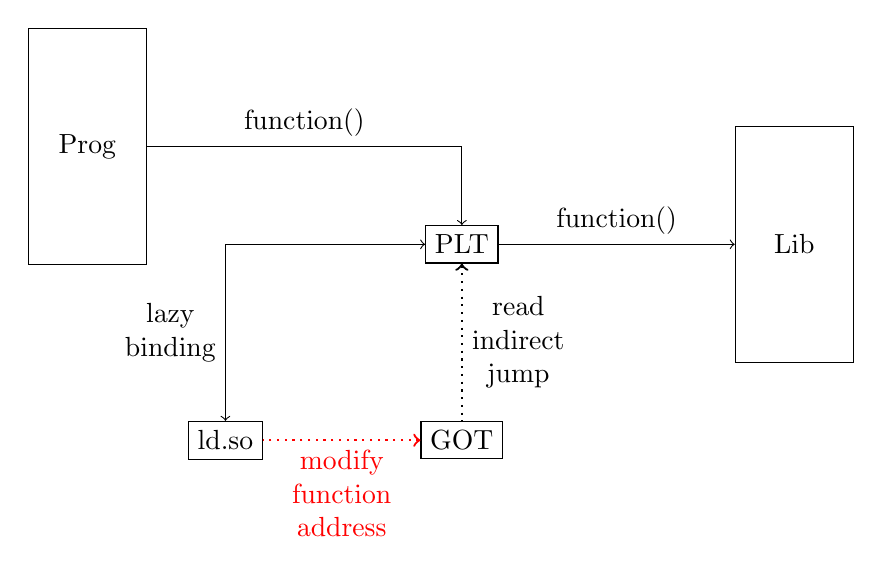
\begin{tikzpicture}
\draw
    node [draw,minimum height=3cm,minimum width=1.5cm] (prog) {Prog};
\draw (prog.east) [->] -- ++(4,0) node [midway,above] {function()} -- ++(0,-1)
    node [draw,below] (plt) {PLT};
\draw (plt.south) [<-,dotted,thick] -- ++(0,-2)
    node [midway,right,align=center] {read\\ indirect\\ jump}
    node [draw,solid,thin,below] (got) {GOT};
in ld.so \draw (got.west) [<-,dotted,thick,red] -- ++(-2,0)
    node [midway,below,align=center] {modify\\ function\\ address}
    node [draw,solid,thin,left,black] (ldso) {ld.so};
\draw (plt.west) [<->] -| 
    node [near end,left,align=center] {lazy\\ binding} (ldso);
\draw (plt.east) [->] -- ++(3,0) node [midway,above] {function()}
    node [draw,right,minimum height=3cm,minimum width=1.5cm] (lib) {Lib};
\end{tikzpicture}
\end{frame}

\subsection{Dangerous PLT GOT}
\begin{frame}{Dangerous PLT GOT}
\begin{itemize}
    \item Procedure Linkage Table
    \item Global Offset Table
    \item writeable table of code pointers
    \item mprotect(2) in ld.so is another gadget
\end{itemize}
\end{frame}

\subsection{kbind(2) System Call}
\begin{frame}{kbind(2) System Call}
\begin{itemize}
    \item modifies single GOT entry
    \item implicit atomic mprotect(2)
    \item can only called from ld.so(1)
    \item protected by data cookie
\end{itemize}
\end{frame}

\section{pledge(2)}

\subsection{pledge(2) Motivation}
\begin{frame}{pledge(2) Motivation}
\begin{itemize}
    \item restrict system calls
    \item declare functional requirements
    \item tool for programmer
    \item abort process at violation
    \item log problems or attacks
\end{itemize}
\end{frame}

\subsection{Way to pledge(2)}
\begin{frame}{Way to pledge(2)}
\begin{itemize}
    \item studdy existing programs
    \item pattern initialization and main loop
    \item design classes of promises
    \item reimplement some libc functions
    \item pledge nearly all programs
\end{itemize}
\end{frame}

\subsection{pledge(2) Consequences}
\begin{frame}{pledge(2) Consequences}
\begin{itemize}
    \item cleanup program flow
    \item delete (mis-)features
    \item design security model
\end{itemize}
\end{frame}

\section{Virtual Address Layout}

\subsection{fork+exec}
\begin{frame}{fork+exec}
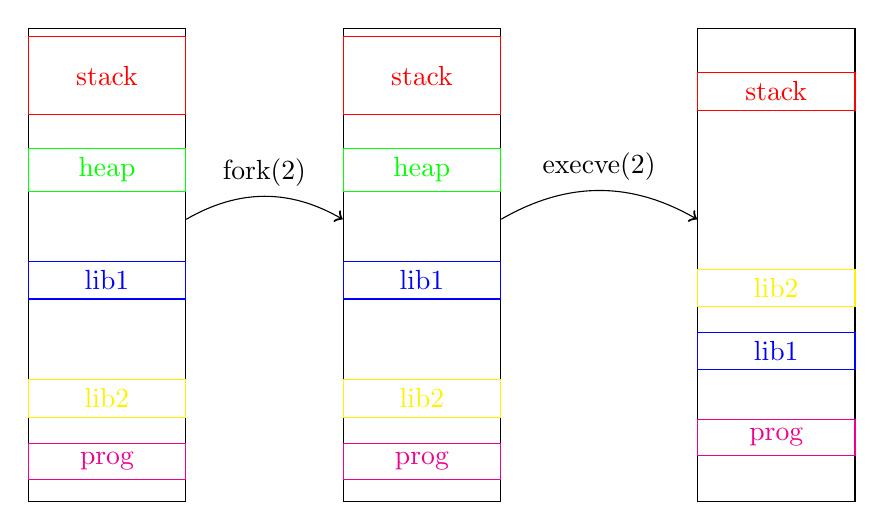
\begin{tikzpicture}
\draw
    (0,0) node [draw,below,minimum width=2cm,minimum height=6cm] (p) {}
    +(0,-0.6) node [draw,minimum width=2cm,red,minimum height=1cm] {stack}
    +(0,-1.8) node [draw,minimum width=2cm,green] {heap}
    +(0,-3.2) node [draw,minimum width=2cm,blue] {lib1}
    +(0,-4.7) node [draw,minimum width=2cm,yellow] {lib2}
    +(0,-5.5) node [draw,minimum width=2cm,magenta] {prog};
\draw
    (4,0) node [draw,below,minimum width=2cm,minimum height=6cm] (f) {}
    +(0,-0.6) node [draw,minimum width=2cm,red,minimum height=1cm] {stack}
    +(0,-1.8) node [draw,minimum width=2cm,green] {heap}
    +(0,-3.2) node [draw,minimum width=2cm,blue] {lib1}
    +(0,-4.7) node [draw,minimum width=2cm,yellow] {lib2}
    +(0,-5.5) node [draw,minimum width=2cm,magenta] {prog};
\draw
    (8.5,0) node [draw,below,minimum width=2cm,minimum height=6cm] (e) {}
    +(0,-0.8) node [draw,minimum width=2cm,red] {stack}
    +(0,-3.3) node [draw,minimum width=2cm,yellow] {lib2}
    +(0,-4.1) node [draw,minimum width=2cm,blue] {lib1}
    +(0,-5.2) node [draw,minimum width=2cm,magenta] {prog};
\draw [->] (p) to [thick,bend left,edge label={fork(2)}] (f);
\draw [->] (f) to [thick,bend left,edge label={execve(2)}] (e);
\end{tikzpicture}
\end{frame}

\subsection{Questions}
\begin{frame}{Questions}
\begin{center}
\begin{tikzpicture}
\draw [font=\Huge] node {?};
\end{tikzpicture}
\end{center}
\end{frame}

\subsection{Links}
\begin{frame}{Links}
\url{https://www.openbsd.org/papers/bsdtw.pdf}
\url{https://www.technovelty.org/linux/plt-and-got-the-key-to-code-sharing-and-dynamic-libraries.html}
\url{https://man.openbsd.org/manual/cgi?kbind} XXX
\end{frame}

\end{document}
